% This example is meant to be compiled with lualatex
\PassOptionsToPackage{unicode}{hyperref}
\documentclass[aspectratio=1610, 9pt]{beamer}


\usetheme[
  % ShowTotalFrames,               % show total number of frames in the footline
  % ProgressBar,                     % show progressbar
  % ProgressBarStart=1,            % start progressbar at page 1
]{code}


\usepackage{fontspec}
\usepackage[english]{babel}

\usepackage{fontawesome5}

\usepackage{amsmath}
\usepackage{mathtools}
\usepackage{amssymb}
\usepackage{mleftright}

\usepackage[
  math-style=ISO,
  bold-style=ISO,
  sans-style=italic,
  nabla=upright,
  partial=upright,
  mathrm=sym,
]{unicode-math}
\setmathfont{Fira Math}[Scale=MatchLowercase]

\usepackage[
  locale=UK,
  separate-uncertainty=true,
  per-mode=symbol-or-fraction,
]{siunitx}

\usepackage[
  german=quotes,
  autostyle,
]{csquotes}
\usepackage{xfrac}

\usepackage{tabularray}
\UseTblrLibrary{booktabs, siunitx, varwidth}
\usepackage{threeparttable}

\usepackage{graphicx}

\usepackage[
  compatibility=false,
]{caption}
\usepackage{subcaption}

\usepackage{xcolor}
\usepackage{metalogo}
\usepackage{pdflscape}

\usepackage{fancyvrb}
\usepackage[outputdir=build]{minted2}
\setminted{
  autogobble,
  breaklines,
  stripnl=true,
}
\usemintedstyle{code}

\usepackage[
  theorems,
  many,
]{tcolorbox}

\usepackage{adjustbox}

\usepackage{tikz}
\usetikzlibrary{
  arrows,
  arrows.meta,
  graphs,
  graphdrawing,
  positioning,
  shadows,
  shapes,
}

\usepackage[edges]{forest}

\usepackage[
  shortcuts,
]{extdash}

\usepackage[noframe]{showframe}
\usepackage{bookmark}


\tikzset{
    position label/.style={
       below = 3pt,
       text height = 1.5ex,
       text depth = 1ex
    },
    brace/.style={
     decoration={brace},
     decorate
   }
}

\forestset{
  textfile/.style = {
    execute at begin node=\textcolor{cblack}{\faFile*}\space
  },
  batchfile/.style = {
    execute at begin node=\textcolor{cblack}{\faTerminal}\space
  },
  makefile/.style = {
    execute at begin node=\textcolor{cblack}{\faFile}\space
  },
  pythonfile/.style = {
    execute at begin node=\textcolor{cblack}{\faPython}\space
  },
  opened/.style = {execute at begin node=\textcolor{dircolor}{\faFolderOpen}\space},
  closed/.style = {execute at begin node=\textcolor{dircolor}{\faFolder}\space},
  dir tree/.style = {
    grow'=0,
    font=\ttfamily,
    folder,
    fit=band,
    s sep=5pt,
    before computing xy={l=20pt},
    edge={rounded corners=2pt},
  },
  visible on/.style={
    % for tree={
    /tikz/visible on={#1},
    for children={
      edge={/tikz/visible on={#1}}}
    },
}


% This adds a circle with a picture of your choice in it.
% Usage:
% \roundpic[<optional arguments>, e.g. xshift or yshift]\
% {<radius of the cirlce [cm]>}{<picture width [cm]>}{<path_to_picture>}{x pos}{y pos}{label}
% TO BE PUT INSIDE TIKZ ENVIRONMENT (i.e. \begin{tikzpicture} \roundpic... \end{tikzpicture})
\NewDocumentCommand \roundpic {o o m m m m m o}{%
  \node [%
    circle, draw, minimum size=#3, #1,
    path picture = {%
      \node [#2] at (path picture bounding box.center) {%
        \IfNoValueF{#8}{\hyperlink{#8}\begingroup}
        \includegraphics[#4]{#5}
        \IfNoValueF{#8}{\endgroup}
      };
    }
  ] at (#6, #7) {};
}%

\NewDocumentCommand\sectionslide{m o}{%
  {
  \setbeamertemplate{background} {
    \begin{tikzpicture}[remember picture,overlay]
      \node [anchor=north, yshift=0.25cm] at (current page.north) {
        \reflectbox{\includegraphics[height=\pageheight+0.5cm]{images/sec_img.jpg}}
      };
      \fill[black, path fading=titlefade, fading transform={xscale=.3, xshift=-1.25cm}]
          (current page.north west) ++(0cm,1cm) rectangle (current page.south east);
    \end{tikzpicture}
  }
  \begin{frame}
    \begin{tikzpicture}[remember picture,overlay]
      \node [anchor=east, opacity=0.3] at ([xshift=-15pt]current page.east) {#2};
      \node [font=\bfseries\huge] (title) at (current page.center) {#1};
      \draw [tugreen, line width=1.2pt] (title.south west) -- (title.north west);
    \end{tikzpicture}
  \end{frame}
  }
}

% icon href
\NewDocumentCommand \iref { s m m } {%
  \IfBooleanTF{#1}{
    \href{#2}{{\footnotesize{\faExternalLink*}}\,#3}
  }{
    \href{#2}{{\footnotesize{\faExternalLink*}}\,\texttt{#3}}
  }
}

\NewDocumentCommand \cpp {} {%
  C\nolinebreak\hspace{-.05em}\raisebox{.1ex}{\texttt{+}}\nolinebreak\hspace{-.10em}\raisebox{.1ex}{\texttt{+}}
}

\NewDocumentCommand \src { m O{cblack!50!cwhite} } {
  {\tiny\textcolor{#2}{[#1]}}
}



\xdefinecolor{dircolor}{HTML}{f0c481}


\ExplSyntaxOn

\RenewDocumentEnvironment {block} {m o} {
  \IfValueTF{#2}{
    \begin{tcolorbox}[
      adjusted~title=#1,
      #2,
    ]
  }{
    \begin{tcolorbox}[
      adjusted~title=#1,
    ]
  }
}{
  \end{tcolorbox}
}

\RenewDocumentEnvironment {alertblock} {m o} {
  \IfValueTF{#2}{
    \begin{tcolorbox}[
      adjusted~title=#1,
      colframe=alertred,
      #2,
    ]
  }{
    \begin{tcolorbox}[
      adjusted~title=#1,
      colframe=alertred,
    ]
  }
}{
  \end{tcolorbox}
}

\RenewDocumentEnvironment {exampleblock} {m o} {
  \IfValueTF{#2}{
    \begin{tcolorbox}[
      adjusted~title=#1,
      colframe=blue!80!black,
      #2,
    ]
  }{
    \begin{tcolorbox}[
      adjusted~title=#1,
      colframe=blue!80!black,
    ]
  }
}{
  \end{tcolorbox}
}
\ExplSyntaxOff


\tikzset{
  invisible/.style={opacity=0,text opacity=0},
  visible on/.style={alt={#1{}{invisible}}},
  alt/.code args={<#1>#2#3}{%
    \alt<#1>{\pgfkeysalso{#2}}{\pgfkeysalso{#3}} % \pgfkeysalso doesn't change the path
  },
}

\NewDocumentCommand \rtd {} {\textbf{Read}\emph{the}\textbf{Docs}}



% Put settings here, like
\unimathsetup{
  math-style=ISO,
  bold-style=ISO,
  nabla=upright,
  partial=upright,
  mathrm=sym,
}

\NewDocumentCommand \eg {} {e.\,g.}
\NewDocumentCommand \ie {} {i.\,e.}

\title{Python Packaging}
\subtitle{A Brief Recap of the PYOPP Workshop}

\author[A.~Knierim]{Anno Knierim}
\contact{{\large{\faGithub}}\:aknierim}
\date{July 25, 2025}


\begin{document}

\maketitle

\begin{frame}{Why Even Bother With Packaging?}
  \begin{center}
    \huge\textcolor{ccyan!90!cblack}{\textbf{Packages allow you to share your code, so other people can use it.}}
  \end{center}
  \vspace{2em}
  \textcolor{cpink}{But also\dots}
  \begin{itemize}
    \setlength{\itemsep}{1em}
    \item Helps you keeping your code from breaking
    \item Benefits other people that may have faced a similar problem
    \item Saves time because code can be reused easily
  \end{itemize}
\end{frame}

\begin{frame}{Before We Start: Package and Environment Managers}
  \begin{description}
    \setlength{\itemsep}{1em}
    \item [\iref{https://pypi.org/project/pip/}{pip}] The standard package installer for Python. \texttt{pip} is able to install
      directly from PyPI and other indexes.
    \item [\iref{https://mamba.readthedocs.io/en/latest/}{mamba}] Fast and robust, with cross-platform support. Written in \cpp.
      Allows you to manage multiple, isolated environments. \texttt{mamba} installs from local or remote package repositories, \eg, channels.
    \item [\iref{https://python-poetry.org/}{poetry}] Package installer that is also able to create its own virtual environments.
      Handles dependency resolving better than pip. Works nicely with \texttt{pyproject.toml} files. Allows the use of lock files.
    \item [\iref{https://docs.astral.sh/uv/}{uv}] A new and fast package manager written in {\footnotesize{\faRust}}\,\texttt{Rust}. Can create
      virtual environments, and solves dependencies better and faster than pip. Allows the use of lock files.
  \end{description}
  \begin{center}
    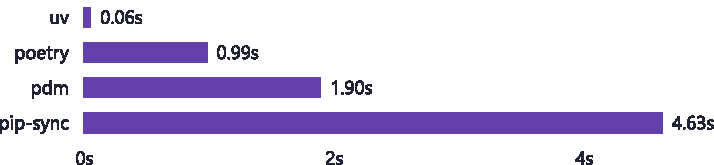
\includegraphics[width=0.7\textwidth]{graphics/speed.pdf}
    \src{docs.astral.sh/uv}
  \end{center}
\end{frame}





\secslide[\fontsize{1.3cm}{1.3cm}\selectfont]{Packaging: The Basics}


\begin{frame}{What Even is a Package?}
  \begin{description}[\texttt{Distribution Package}]
    \setlength{\itemsep}{1.5em}
    \item [\texttt{Import Package}] Any Python module that you can \emph{import} using the \mintinline{python}+import+
      statement.
    \item [\texttt{Namespace Package}] Packages that allow you to \emph{unify} two packages with the \emph{same} name.
    \item [\texttt{Distribution Package}] An archive containing a \emph{collection} of import packages combined with
      \emph{metadata} such as dependencies.
  \end{description}
  \vspace{1cm}
  \uncover<2>{
  \begin{center}
    \huge\textcolor{ccyan}{When people talk about packages, they usually mean \textbf{distribution packages.}}
  \end{center}
  }
\end{frame}

\begin{darkframe}{How Does Python Find Installed Packages?}
  \begin{center}
  \huge\textcolor{ccyan}{Example: NumPy}
  \end{center}
  \vspace{0.5cm}
  \begin{minted}{shell-session}
    $ python -c "import numpy; print(numpy.__path__[0])"
    /home/anno/.local/conda/envs/pyopp_recap/lib/python3.12/site-packages/numpy

    $ ls -C $(python -c "import numpy; print(numpy.__path__[0])") | sort
    _array_api_info.py     doc		      __init__.py	 py.typed
    _array_api_info.pyi    dtypes.py	      __init__.pyi	 random
    char		      dtypes.pyi	      lib		 rec
    __config__.py	      exceptions.py	      linalg		 strings
    __config__.pyi	      exceptions.pyi	      ma		 testing
    _configtool.py	      _expired_attrs_2_0.py   matlib.py	 tests
    _configtool.pyi        _expired_attrs_2_0.pyi  matlib.pyi	 _typing
    conftest.py	      f2py		      matrixlib	 typing
    _core		      fft		      polynomial	 _utils
    core		      _globals.py	      __pycache__	 version.py
    ctypeslib	      _globals.pyi	      _pyinstaller	 version.pyi
    _distributor_init.pyi  __init__.pxd	      _pytesttester.pyi
    _distributor_init.py   __init__.cython-30.pxd  _pytesttester.py
  \end{minted}
\end{darkframe}


\begin{frame}[fragile]{How Do I Create a Package?}
  \begin{center}
    \huge\textcolor{ccyan!90!cblack}{\textbf{There is not \enquote{just one way} to create packages, but\dots}}
  \end{center}
  \vspace{1em}
  \begin{itemize}
    \setlength{\itemsep}{1em}
    \item Modern packaging uses a scaffolding called \texttt{pyproject.toml} with three important sections:
    \begin{description}[\texttt{[build-system]}]
      \item [\mintinline{toml}{[build-system]}] Allows you to describe what build backend to use.
      \item [\mintinline{toml}{[project]}] Sets up metadata for the package, such as the name or version.
      \item [\mintinline{toml}{[tool]}] A section for tool configuration.
    \end{description}
    \item An easy way to set up that scaffolding: \href{https://hatch.pypa.io/latest/}{{\footnotesize{\faExternalLink*}}\,\texttt{hatch}}
      \begin{minted}{shell-session}
        $ uv pip install hatch
        $ mamba install hatch
      \end{minted}
  \end{itemize}
\end{frame}

\begin{splitframe}[fragile]{How Do I Create a Package?}{Output}
  \begin{columns}[t,onlytextwidth]
    \begin{column}{0.58\textwidth}
      \begin{itemize}
        \item Use \textcolor{cpink}{\texttt{hatch}}'s CLI tool to quickstart creating a package:
          \begin{minted}{shell-session}
            $ hatch new my_package
          \end{minted}
      \end{itemize}
    \end{column}
    \hfill
    \begin{column}{0.38\textwidth}
      \begin{minted}{toml}
        my_package
        ├── src
        │   └── my_package
        │       ├── __about__.py
        │       └── __init__.py
        ├── tests
        │   └── __init__.py
        ├── LICENSE.txt
        ├── README.md
        └── pyproject.toml
      \end{minted}
    \end{column}
  \end{columns}
  \vspace{1em}
  \begin{columns}[t,onlytextwidth]
    \begin{column}{0.58\textwidth}
      \begin{itemize}
        \setlength{\itemsep}{1em}
        \item Let's see what this created:
          \begin{minted}{shell-session}
            $ head my_package/pyproject.toml
          \end{minted}
        \item You can also upgrade an existing project to use \texttt{hatch}:
          \begin{minted}{shell-session}
            $ hatch new --init
          \end{minted}
        \item Have a look at the \href{https://packaging.python.org/en/latest/guides/writing-pyproject-toml/}{{\footnotesize{\faExternalLink*}}\,Writing your \texttt{pyproject.toml}}
          guide to learn how to customise the \texttt{pyproject.toml} file
      \end{itemize}
    \end{column}
    \begin{column}{0.38\textwidth}
      \begin{minted}{toml}
        [build-system]
        requires = ["hatchling"]
        build-backend = "hatchling.build"

        [project]
        name = "my_package"
        dynamic = ["version"]
        description = ''
        readme = "README.md"
        requires-python = ">=3.8"
      \end{minted}
    \end{column}
  \end{columns}
\end{splitframe}

\begin{splitframe}[fragile]{Dependencies}{Example}
  \begin{columns}[t,onlytextwidth]
    \begin{column}{0.58\textwidth}
      \begin{itemize}
        \setlength{\itemsep}{1em}
        \item Dependencies for your project are defined with the \texttt{dependencies}
          key inside the \texttt{[project]} section
        \item You can set \href{https://packaging.python.org/en/latest/specifications/dependency-specifiers/}{{\footnotesize{\faExternalLink*}}\,dependency specifiers}
          (aka constraints) such as versions
      \end{itemize}
    \end{column}
    \hfill
    \begin{column}{0.38\textwidth}
      \begin{minted}{toml}
        [project]
        dependencies = [
          "numpy",
          "astropy<=6.1.0",
          "tomli;python_version<'3.11'",
        ]
      \end{minted}
    \end{column}
  \end{columns}
  \vspace{1em}
  \begin{columns}[t,onlytextwidth]
    \begin{column}{0.58\textwidth}
      \begin{itemize}
        \setlength{\itemsep}{1em}
        \item Define your optional dependencies in the \texttt{[project.optional-dependencies]} section
          and group them
        \item Install optional dependencies using
          {
          \usemintedstyle{code-light}
          \begin{minted}{shell-session}
            $ uv pip install my_package[plot]
            $ uv pip install "my_package[plot]"
          \end{minted}
          }
      \end{itemize}
    \end{column}
    \hfill
    \begin{column}{0.38\textwidth}
      \begin{minted}{toml}
        [project.optional-dependencies]
        plot = ["matplotlib"]
      \end{minted}
    \end{column}
  \end{columns}
  \vspace{1em}
\end{splitframe}

\begin{splitframe}[fragile]{Dependency Groups}{Example}
  \begin{columns}[t,onlytextwidth]
    \begin{column}{0.58\textwidth}
      \begin{itemize}
        \setlength{\itemsep}{1em}
        \item Fairly new (accepted \texttt{2024-10-10}): \href{https://peps.python.org/pep-0735/}{{\footnotesize{\faExternalLink*}}\,\texttt{PEP 735}} Dependency Groups
        \item Optional dependencies that are \emph{not} installed when a \emph{user} installs the package, \eg, via PyPI
          \begin{itemize}
            \item [\to] Prevent users from installing dev tools
          \end{itemize}
        \item Install the groups from within your source repo:
          \begin{minted}{shell-session}
            $ uv pip install --group dev
          \end{minted}
      \end{itemize}
    \end{column}
    \hfill
    \begin{column}{0.38\textwidth}
      \begin{minted}{toml}
        [dependency-groups]
        tests = ["pytest", "pytest-cov"]
        docs = ["sphinx"]
        dev = [
          "jupyter",
          "pre-commit",
          {include-group = "tests"},
          {include-group = "docs"},
        ]
      \end{minted}
    \end{column}
  \end{columns}
\end{splitframe}

\secslide{Code Quality}

\begin{darkframe}
  \begin{center}
    \uncover<2>{
      
\includegraphics[width=0.35\textwidth]{graphics/patrick.jpg}
    }
    \\[1.5em]
    \begin{minipage}{0.8\textwidth}
      \begin{minted}{python}
        def f(x,y=0):return[x[i]+y if x[i]>0else y-x[i]for i in range(len(x))]
      \end{minted}
    \end{minipage}
    \\[3em]
    \uncover<2>{
      \huge\textcolor{ccyan}{This runs, but do you trust it?}
    }
  \end{center}

  \begin{tikzpicture}[remember picture, overlay]
    \coordinate (pos) at ([xshift=-2cm, yshift=1cm]current page.south east);
    \node [rotate around={30:(pos)}, align=center] at (pos) {Shamelessly taken from\\Stefan's talk :)};
  \end{tikzpicture}
\end{darkframe}

\begin{darkframe}{Code Quality Terminology}
  \Huge
  \begin{enumerate}
    \setlength{\itemsep}{2em}
    \item \textcolor{ccyan}{Surface Quality}
      \begin{itemize}
        \item [\to] Formatting: Layout, naming conventions, whitespaces
      \end{itemize}
    \item \textcolor{ccyan}{Semantic Quality}
      \begin{itemize}
        \item [\to] Docstrings, type hinting
      \end{itemize}
    \item \textcolor{ccyan}{Testability}
      \begin{itemize}
        \item [\to] Writing (simple) code that is easy to test
      \end{itemize}
  \end{enumerate}
\end{darkframe}

\begin{frame}{Surface Quality: PEP 8}
  \begin{center}
    \huge\iref{https://peps.python.org/pep-0008/}{Python Enhancement Proposal No. 8 (PEP 8)}
  \end{center}
  \begin{itemize}
    \setlength{\itemsep}{1em}
    \item Coding convention comprising the standard library, all about readability
    \item Key Aspects:\\
      \begin{center}
      \begin{tblr}{
          colspec={c c c},
          rows={font=\bfseries\Large, fg=ccyan, rowsep=0.25cm},
          columns={colsep=0.75cm},
        }
        Code Layout & String Quotes & Whitespaces \\
        Trailing Commas & Comments & Naming Conventions
      \end{tblr}
      \end{center}
  \end{itemize}
\end{frame}

\begin{darkframe}[fragile]{Surface Quality: PEP 8}
  \begin{center}
    \begin{tikzpicture}[remember picture]
      \node [anchor=east, outer sep=10pt] (wrong) at ([xshift=-1cm]current page.center) {
      \begin{minipage}{0.3\textwidth}
        \begin{minted}{python}
          def add(a, b): return a+b
          from rich import print
          import os, math
          def printPi():print(math.pi)
        \end{minted}
      \end{minipage}
    };

      \node [anchor=west, outer sep=10pt] (correct) at ([xshift=1cm]current page.center) {
      \begin{minipage}{0.3\textwidth}
        \begin{minted}{python}
          import os, math

          from rich import print


          def add(a, b):
              return a + b


          def print_pi():
              print(math.pi)
        \end{minted}
      \end{minipage}
    };

      \draw [->, >=latex] (wrong) -- (correct);
  \end{tikzpicture}
  \end{center}
\end{darkframe}

\begin{frame}{Surface Quality: Tools}
  \large
  \begin{description}[\iref{https://pycodestyle.pycqa.org/en/latest/}{pycodestyle}]
    \setlength{\itemsep}{1em}
    \item [\iref{https://pycodestyle.pycqa.org/en/latest/}{pycodestyle}] Strict \texttt{PEP8} formatter.
    \item [\iref{https://flake8.pycqa.org/en/latest/}{flake8}] \texttt{pyflakes} + \texttt{pycodestyle} + \texttt{optional plugins}.
    \item [\iref{https://black.readthedocs.io/en/stable/}{black}] Follows \texttt{PEP8} and adds it's
      own strict rules (\eg, 88 chars limit).
    \item [\iref{https://pycqa.github.io/isort/}{isort}] Sorts imports so you don't have to.
    \item [\iref{https://docs.astral.sh/ruff/}{Ruff}] All of the above, highly customizable using
      \texttt{pyproject.toml} or \texttt{ruff.toml}, and extremely fast.
  \end{description}
  \vspace{0.5cm}
  \begin{center}
    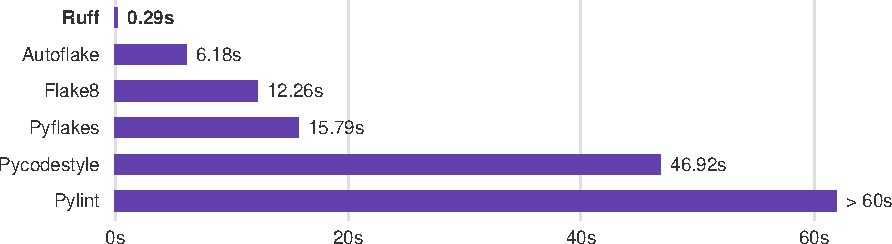
\includegraphics[width=0.7\textwidth]{graphics/speed_ruff.pdf}\src{docs.astral.sh/ruff}
  \end{center}
\end{frame}

\begin{splitframe}[fragile]{Surface Quality: Ruff}{pyproject.toml}
  \begin{columns}[t,onlytextwidth]
    \begin{column}{0.58\textwidth}
      {
      \usemintedstyle{code-light}
      \begin{itemize}
        \setlength{\itemsep}{2.5em}
        \item Install via \texttt{uv} as global tool or add to your project:
          \begin{minted}{shell-session}
            $ uv tool install ruff@latest
            $ uv add --dev ruff
          \end{minted}
        \item Two tools in one: \emph{Formatter} and \emph{linter}
          \begin{minted}{shell-session}
            $ ruff check
            $ ruff format
          \end{minted}
        \item Ruff supports over \emph{800} lint rules, inspired by the popular tools
          shown earlier \to{} See \iref{https://docs.astral.sh/ruff/rules/}{Rules}.
          \begin{itemize}
            \setlength{\itemsep}{1em}
            \item [\to] Configure everything in \texttt{pyproject.toml} or \texttt{ruff.toml}.
            \item [\to] Disable specific rules that you don't need in your project, \eg, \texttt{B905} \textit{zip-without-explicit-strict}.
          \end{itemize}
      \end{itemize}
      }
    \end{column}
    \hfill
    \begin{column}{0.38\textwidth}
      \footnotesize
      \vspace*{0.25cm}
      \begin{minted}{toml}
        [tool.ruff]
        target-version = "py313"
        line-length = 88
        extend-exclude = ["tests"]

        [tool.ruff.lint]
        extend-select = [
          "I",   # isort
          "E",   # pycodestyle
          "F",   # Pyflakes
          "UP",  # pyupgrade
          "B",   # flake8-bugbear
          "SIM", # flake8-simplify
        ]
        ignore = ["B905"]

        fixable = ["ALL"]
        unfixable = []

        [tool.ruff.lint.per-file-ignores]
        "examples/**" = ["I"]

        [tool.ruff.format]
        quote-style = "double"
        indent-style = "space"
        line-ending = "auto"
        skip-magic-trailing-comma = false
        docstring-code-format = true

        [tool.ruff.lint.isort]
        known-first-party = ["my_package"]
      \end{minted}
    \end{column}
  \end{columns}
\end{splitframe}

\begin{splitframe}[fragile]{Semantic Quality: Docstrings}{NumPy Style}
  \begin{columns}[t,onlytextwidth]
    \begin{column}{0.58\textwidth}
      {
      \usemintedstyle{code-light}
      \begin{itemize}
        \setlength{\itemsep}{2.5em}
        \item Explains what your code does.
        \item Can be understood by IDEs and autocompletion tools
        \item Necessary for well-written docs (later)
        \item Structure:
          \begin{itemize}
            \item [\to] Triple double quotes (\mintinline{python}+"""..."""+)
            \item Human-readable, complete sentences describing your code
            \item Explanation of parameters, returns, and exceptions
          \end{itemize}
        \item Many different styles available: Use \emph{one} and \emph{stick to it}.
      \end{itemize}
      }
    \end{column}
    \hfill
    \begin{column}{0.38\textwidth}
      \footnotesize
      \vspace*{0.25cm}
      \begin{minted}{python}
        def draw_sampling_opts(size: int) -> Dict:
            """Draws randomized sampling parameters
            for the simulation.

            Parameters
            ----------
            size : int
                Number of parameters to draw, equal
                to number of images.

            Returns
            -------
            samp_opts : dict
                Sampling options/parameters stored
                inside a dictionary.
            """
      \end{minted}
    \end{column}
  \end{columns}
\end{splitframe}

{
\usemintedstyle{code-light}
\begin{frame}[fragile]{Semantic Quality: Type Hinting}
  \begin{center}
    \huge\textcolor{ccyan}{Python is dynamically typed, but\dots}
  \end{center}
  \begin{itemize}
    \setlength{\itemsep}{1em}
    \item \dots you can still declare types for variables:
      \begin{minted}{python}
        foo: int = 1
        bar: str = "app"
        baz: np.ndarray = np.array([...])

        def func(a: int, b: int=42) -> int:
          return a + b
      \end{minted}
    \item [\to] Improved code readability
    \item IDE and linting support, \eg, through code completion
    \item But: Type hinting is \emph{not} enforced at runtime and one has
      to consider dynamic types

    \item Tools:
      \begin{description}[\iref{https://microsoft.github.io/pyright/}{pyright}]
        \item [\iref{https://mypy-lang.org/}{mypy}] Good for CI/CLI
        \item [\iref{https://microsoft.github.io/pyright/}{pyright}] Proprietary tool, but faster and with VSCode integration
      \end{description}
  \end{itemize}
\end{frame}
}

\begin{splitframe}[fragile]{Automation: pre-commit Hook}{.pre-commit-config.yaml}{0.5}
  \begin{columns}[t,onlytextwidth]
    \begin{column}{0.48\textwidth}
      {
      \usemintedstyle{code-light}
      \begin{itemize}
        \setlength{\itemsep}{2em}
        \item \iref{https://pre-commit.com/}{pre-commit} does all the formatting and linting for you
        \item Install via \texttt{uv}:
          \begin{minted}{shell-session}
            $ uv pip install pre-commit
          \end{minted}
        \item Many different hooks available:
          \begin{itemize}
            \item \texttt{ruff}, \texttt{mypy}, \iref{https://github.com/codespell-project/codespell}{codespell}, and many more\dots
          \end{itemize}
        \item Runs all tools defined in \texttt{.pre-commit-config.yaml}
        \item Run \mintinline{shell-session}+$ pre-commit install+ to install
          hooks in your project
        \item \mintinline{shell-session}{pre-commit} runs automatically whenever something is comitted
          using \mintinline{shell-session}{$ git commit ...}
      \end{itemize}
      }
    \end{column}
    \hfill
    \begin{column}{0.48\textwidth}
      \footnotesize
      \vspace*{0.25cm}
      \begin{minted}{yaml}
        repos:
          - repo: https://github.com/pre-commit/pre-commit-hooks
            rev: "v5.0.0"  # <- git version tag
            hooks:
              - id: check-added-large-files
              - id: check-case-conflict
              - id: check-merge-conflict
              - id: check-symlinks
              - id: check-yaml
              - id: debug-statements
              - id: end-of-file-fixer
              - id: mixed-line-ending
              - id: name-tests-test
                args: ["--pytest-test-first"]
              - id: requirements-txt-fixer
              - id: trailing-whitespace

          - repo: https://github.com/astral-sh/ruff-pre-commit
            rev: "v0.12.3"
            hooks:
              - id: ruff-format
              - id: ruff-check
                args: ["--fix", "--show-fixes"]

          - repo: https://github.com/codespell-project/codespell
            rev: v2.4.1
            hooks:
            - id: codespell
              additional_dependencies:
                - tomli
      \end{minted}
    \end{column}
  \end{columns}
\end{splitframe}

\begin{frame}{Further Reading: Code Quality}
  \begin{itemize}
    \setlength{\itemsep}{1em}
    \item \iref{https://indico.desy.de/event/43817/sessions/19711/attachments/97900/134904/Code\%20Quality\%20PYOPP.pdf}{Stefans Talk On Code Quality}
    \item \iref{https://peps.python.org/pep-0008/}{Python Enhancement Proposal No. 8 (PEP 8)}
    \item \iref{https://docs.astral.sh/ruff/}{Ruff Docs}
    \item \iref{https://mypy.readthedocs.io/en/stable/}{mypy Docs}
    \item \iref{https://microsoft.github.io/pyright/}{pyright Docs}
    \item \iref{https://pre-commit.com/}{pre-commit}
    \item \iref{https://github.com/pre-commit/pre-commit-hooks}{pre-commit-hooks}
    \item \iref{https://github.com/codespell-project/codespell}{codespell}
  \end{itemize}
\end{frame}

\secslide{Testing}

\begin{frame}{When Do We Need Tests?}
  \begin{center}
    \huge\textcolor{ccyan!90!cblack}{Imagine the following\dots}
  \end{center}
  \begin{itemize}
    \item You have written a package with a lot of code, \eg, multiple scripts
    \item You found a bug somewhere in your code
    \item You have not thought of possible edge cases during development
  \end{itemize}
  \vspace{1em}
  \begin{center}
    \huge\textcolor{cpink!90!cblack}{\to{} You will need to investigate your codebase for
    causes of the bug and even then the same bug may appear some time later}
  \end{center}
\end{frame}

\begin{frame}{Solution}
  \begin{center}
    \huge\textcolor{ccyan!90!cblack}{Write persistent tests \textbf{during development!}}\\
    \uncover<2>{\huge\textcolor{ccyan!90!cblack}{(And \textbf{automate} them \to{} see CI)}}

    \begin{tikzpicture}[remember picture, overlay]
      \only<2>{
        \node [anchor=south] at ([yshift=1cm]current page.south) {
          
\includegraphics[height=3cm]{graphics/automation_meme.png}
        };
      }
    \end{tikzpicture}
  \end{center}
\end{frame}

\begin{frame}{Test Levels}
  \begin{description}[Operational Acceptance Testing]
    \setlength{\itemsep}{1em}
    \item [Unit Testing] Test single units (\ie, single functions or classes) of your software.
    \item [Integration Testing] Test multiple components that depend on each other.
    \item [System Testing] Test the entire software with respect to its requirements, \eg, I/O data.
    \item [Operational Acceptance Testing] Give your software to the user to break it.
  \end{description}
  \vspace{0.5cm}
  \uncover<2>{
    \begin{center}
      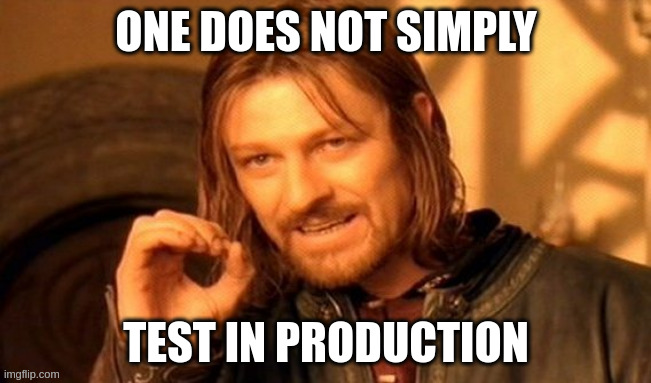
\includegraphics[height=3cm]{graphics/onedoesnot.jpg}
    \end{center}
  }
\end{frame}

\begin{frame}{What Do We Test For?}
  \begin{center}
    \huge\textcolor{ccyan}{This is probably the hardest part\dots}
  \end{center}
  \begin{itemize}
    \setlength{\itemsep}{1em}
    \item You will need to understand your code
    \item You will need to verify how much and what parts of your code are covered by tests
    \item Even then your code may not be guaranteed to work error-free
    \item \emph{Good practice}: Every time you find a bug, add a unit test so it doesn't reappear
  \end{itemize}
\end{frame}

\begin{frame}{Tools}
  Shipped with Python:
  \begin{description}
    \item [\iref{https://docs.python.org/3/library/doctest.html}{doctest}] Allows you to write simple tests in the docstrings
      of your functions.
    \item [\iref{https://docs.python.org/3/library/unittest.html}{unittest}] Allows you to write regular unit tests,
      \ie, separate functions and classes that test your code.
  \end{description}
  \vspace{0.5cm}
  Further tools:
  \begin{description}
    \item [\iref{https://docs.pytest.org/en/stable/}{pytest}] Scalable, and easy to use test framework.
  \end{description}
\end{frame}

\secslide{Documentation}

\begin{frame}{Why Should We Document Our Code?}
  \begin{center}
    \huge\textcolor{ccyan!90!cblack}{Well documented code improves\dots}
  \end{center}
  \begin{itemize}
    \item Maintainability: Future developers, debugging, \dots
    \item Accessibility: Make your package easier to understand for new users
    \item Collaboration: Docs as a shared knowledge source
  \end{itemize}
\end{frame}

\begin{frame}[fragile]{Tool Of Choice: Sphinx}
  \begin{columns}[t, onlytextwidth]
    \begin{column}{0.68\textwidth}
      \begin{itemize}
        \setlength{\itemsep}{1em}
        \item FOSS, extensible documentation generator written in Python
        \item Multiple output formats: \texttt{HTML}, \LaTeX, ePub, and more\dots
        \item Content is written using a mark-up language (\texttt{reST} or \texttt{MyST})
        \item Support for various docstring formats (some through extensions)
        \item Install via uv or mamba:
          \begin{minted}{text}
            $ uv pip install sphinx
            $ mamba install sphinx
          \end{minted}
      \end{itemize}
    \end{column}
    \hfill
    \begin{column}{0.38\textwidth}
      \begin{center}
      
\includegraphics[width=0.8\textwidth]{logos/sphinx-logo.pdf}
      \end{center}
    \end{column}
  \end{columns}
\end{frame}


\begin{frame}[fragile]{Getting Started}
  \begin{minted}[escapeinside=||]{shell-session}
    $ sphinx-quickstart docs
    |\textcolor{ccyan}{> Separate source and build directories (y/n) [n]:}| y
    |\textcolor{ccyan}{> Project name:}| ...
    |\textcolor{ccyan}{> Author name(s):}| ...
    |\textcolor{ccyan}{> Project release []:}| ...
    |\textcolor{ccyan}{> Project language [en]:}| ...
  \end{minted}

  \begin{center}
  \pause
  \begin{minipage}{.45\textwidth}
  \adjustbox{max height=5.5cm}{%
    \begin{forest}
      for tree={dir tree}
      [docs, opened
        [build, closed]
        [source, opened
          [\_static, closed]
          [\_templates, closed]
          [conf.py, pythonfile]
          [index.rst, textfile]
        ]
        [make.bat, batchfile]
        [Makefile, makefile]
      ]
    \end{forest}
  }
  \end{minipage}
  \hfill
  \pause
  \begin{minipage}{.45\textwidth}
    \adjustbox{max height=5.5cm}{%
      \begin{forest}
        for tree={dir tree}
        [docs, opened
          [\_build, closed]
          [\_static, closed]
          [\_templates, closed]
          [conf.py, pythonfile]
          [index.rst, textfile]
          [make.bat, batchfile]
          [Makefile, makefile]
        ]
      \end{forest}
    }
  \end{minipage}
  \end{center}
\end{frame}

{
\setbeamercolor{description item}{fg=cblack}
\begin{frame}[fragile]{Breakdown of the Generated Structure}
  \begin{description}[labelwidth=\widthof{\faFolderOpen \texttt{\_templates}}]
    \setlength{\itemindent}{-4em}
    \item [\textcolor{dircolor}{\faFolderOpen} \texttt{build}:] Output directory for the docs.
    \item [\textcolor{dircolor}{\faFolderOpen} \texttt{\_static}:] Directory for static elements such as images, icons, or logos.
    \item [\textcolor{dircolor}{\faFolderOpen} \texttt{\_templates}:] Used to store \iref{https://jinja.palletsprojects.com/en/stable/}{\texttt{Jinja}}
      templates for HTML page generation. %Also used by some Sphinx extensions.
    \item [\faFile* \texttt{index.rst}:] Root document; contains the root of the table of contents tree.
      % Effectively your landing page in the HTML version.
    \item [\faPython \texttt{conf.py}:] Main configuration file written in Python.
  \end{description}
\end{frame}
}

{
\usemintedstyle{code-light}
\begin{frame}[fragile]{Let's Build Our Docs}
  We will use the \texttt{Makefile} generated by \mintinline{shell-session}+sphinx-quickstart+ to build any format:
  \begin{minted}{shell-session}
    $ make <format>
  \end{minted}
  So, for the HTML version:
  \begin{minted}{shell-session}
    $ make html
  \end{minted}
  This will generate the HTML files for our docs inside the \texttt{build} directory.
  We can view the docs locally by running a Python HTTP server (in this case from inside the \texttt{docs} directory):
  \begin{minted}{shell-session}
    $ python -m http.server -d build/html [port]
  \end{minted}

  \begin{block}{Note}
    \mintinline{shell-session}+[port]+ is optional, see \mintinline{shell-session}+python -m http.server --help+.
  \end{block}
\end{frame}
}


\end{document}
